\documentclass[a4paper,12pt]{article} % добавить leqno в [] для нумерации слева
\usepackage[a4paper,top=1.3cm,bottom=2cm,left=1.5cm,right=1.5cm,marginparwidth=0.75cm]{geometry}
%%% Работа с русским языком
\usepackage{cmap}					% поиск в PDF
\usepackage[warn]{mathtext} 		% русские буквы в фомулах
\usepackage[T2A]{fontenc}			% кодировка
\usepackage[utf8]{inputenc}			% кодировка исходного текста
\usepackage[english,russian]{babel}	% локализация и переносы
\usepackage{physics}
\usepackage{multirow}

%%% Нормальное размещение таблиц (писать [H] в окружении таблицы)
\usepackage{float}
\restylefloat{table}


\usepackage{graphicx}

\usepackage{wrapfig}
\usepackage{tabularx}

\usepackage{hyperref}
\usepackage[rgb]{xcolor}
\hypersetup{
	colorlinks=true,urlcolor=blue
}

%%% Дополнительная работа с математикой
\usepackage{amsmath,amsfonts,amssymb,amsthm,mathtools} % AMS
\usepackage{icomma} % "Умная" запятая: $0,2$ --- число, $0, 2$ --- перечисление

%% Номера формул
%\mathtoolsset{showonlyrefs=true} % Показывать номера только у тех формул, на которые есть \eqref{} в тексте.

%% Шрифты
\usepackage{euscript}	 % Шрифт Евклид
\usepackage{mathrsfs} % Красивый матшрифт
\usepackage{pgfplots}
\pgfplotsset{compat=1.9}

%% Свои команды
\DeclareMathOperator{\sgn}{\mathop{sgn}}

%% Перенос знаков в формулах (по Львовскому)
\newcommand*{\hm}[1]{#1\nobreak\discretionary{}
	{\hbox{$\mathsurround=0pt #1$}}{}}

\date{\today}

\begin{document}

\begin{titlepage}
	\begin{center}
		{\large МОСКОВСКИЙ ФИЗИКО-ТЕХНИЧЕСКИЙ ИНСТИТУТ (НАЦИОНАЛЬНЫЙ ИССЛЕДОВАТЕЛЬСКИЙ УНИВЕРСИТЕТ)}
	\end{center}
	\begin{center}
		{\large Физтех-школа физики и исследований им. Ландау}
	\end{center}
	
	
	\vspace{4.5cm}
	{\huge
		\begin{center}
			{\bf Отчёт о выполнении лабораторной работы №3.4.1}\\
			Измерение магнитной восприимчивости диа- и пара- магнетиков
		\end{center}
	}
	\vspace{2cm}
	\begin{flushright}
		{\LARGE Автор:\\ Сенокосов Арсений Олегович \\
			\vspace{0.2cm}
			Б02-012}
	\end{flushright}
	\vspace{8cm}
	\begin{center}
		Долгопрудный\\
		\today
	\end{center}
\end{titlepage}

\section{Введение}

\textbf{Цель работы:} измерение магнитной восприимчивости диа- и пара- магнетиков.
\\
\textbf{В работе используются:} электромагнит, весы, милливеберметр, регулируемый источник постоянного тока, образцы диа- и парамагнетиков.

\section{Теоретические сведения}

Магнитная восприимчивость тел может быть определена методом измерения сил, которые действуют на тела в магнитном поле. Существуют два классических метода таких измерений: метод Фарадея и метод Гюи. В методе Фарадея исследуемые образцы, имеющие форму маленьких шариков, помещаются в область сильно неоднородного магнитного поля и измеряется сила, действующая на образец. При этом для расчёта магнитной восприимчивости необходимо знать величину градиента магнитного поля в месте расположения образца. В методе Гюи используется тонкий и длинный стержень, один из концов которого помещают в зазор электромагнита (обычно в область однородного поля), а другой конец -- вне зазора, где величиной магнитного поля можно пренебречь. Закон изменения поля -- от максимального до нулевого -- в этом случае несуществен.

Найдём выражение для магнитной силы, действующей на такой образец (рис. \ref{pic:2}). Пусть площадь образца равна $ s $, его магнитная проницаемость -- $ \mu $, а поле в зазоре равно $ B $.

\begin{wrapfigure}{r}{4cm}
	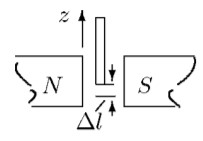
\includegraphics[width=4cm]{Screenshot_2.jpg}
	\caption{Расположение образца в зазоре электромагнита}
	\label{pic:2}
\end{wrapfigure}

Воспользуемся для расчёта энергетическими соображениями. Магнитная сила может быть вычислена как производная от магнитной энергии по перемещению. Из теории известно, что эту производную следует брать со знаком минус, когда образец находится в поле постоянного магнита, или со знаком плюс, как в нашем случае, когда поле в зазоре создаётся электромагнитом, ток $ I $ в обмотках которого поддерживается постоянным.

При смещении образца на расстояние $ \Delta l $ вниз магнитная сила, действующая на него, равна

\begin{equation}\label{1}
F = \left(\frac{\Delta W_m}{\Delta l}\right)_I,
\end{equation}
где $ \Delta W_m $ -- изменение магнитной энергии системы при постоянном токе
в обмотке электромагнита и, следовательно, при постоянной величине
магнитного поля в зазоре.

Магнитная энергия рассчитывается по формуле

\begin{equation}\label{2}
W_m=\frac{1}{2}\int HBd\,V = \frac{1}{2\mu_0}\int\frac{B^2}{\mu}d\,V,
\end{equation}
где интеграл распространён на всё пространство. При смещении образца магнитная энергия меняется только в области зазора (в объёме площади $ s $ и высоты $ \Delta l $), а около верхнего конца стержня остаётся неизменной, поскольку магнитного поля там практически нет. Принимая поле внутри стержня равным измеренному нами полю в зазоре $ B $, получим

\begin{equation}\label{3}
\Delta W_m=\frac{1}{2\mu_0}\frac{B^2}{\mu}s\Delta l - \frac{1}{2\mu_0}B^2 s\Delta l = -\frac{\chi}{2\mu_0\mu}B^2s\Delta l.
\end{equation}

Следовательно, на образец действует сила

\begin{equation}\label{4}
F = -\frac{\chi}{2\mu_0\mu}B^2s.
\end{equation}

Знак силы, действующей на образец, зависит от знака $ \chi $: образцы из парамагнитных материалов $( \chi  > 0)$ втягиваются в зазор электромагнита, а диамагнитные образцы $ (\chi < 0) $ выталкиваются из него.

Пренебрегая отличием $ \mu $ от единицы, получаем окончательно расчётную формулу в виде

\begin{equation}\label{5}
F = -\frac{\chi B^2s}{2\mu_0}.
\end{equation}

Измерив силу, действующую на образец в магнитном поле $ B $, можно рассчитать магнитную восприимчивость образца.

\section{Экспериментальная установка}

\begin{wrapfigure}{r}{6.5cm}
	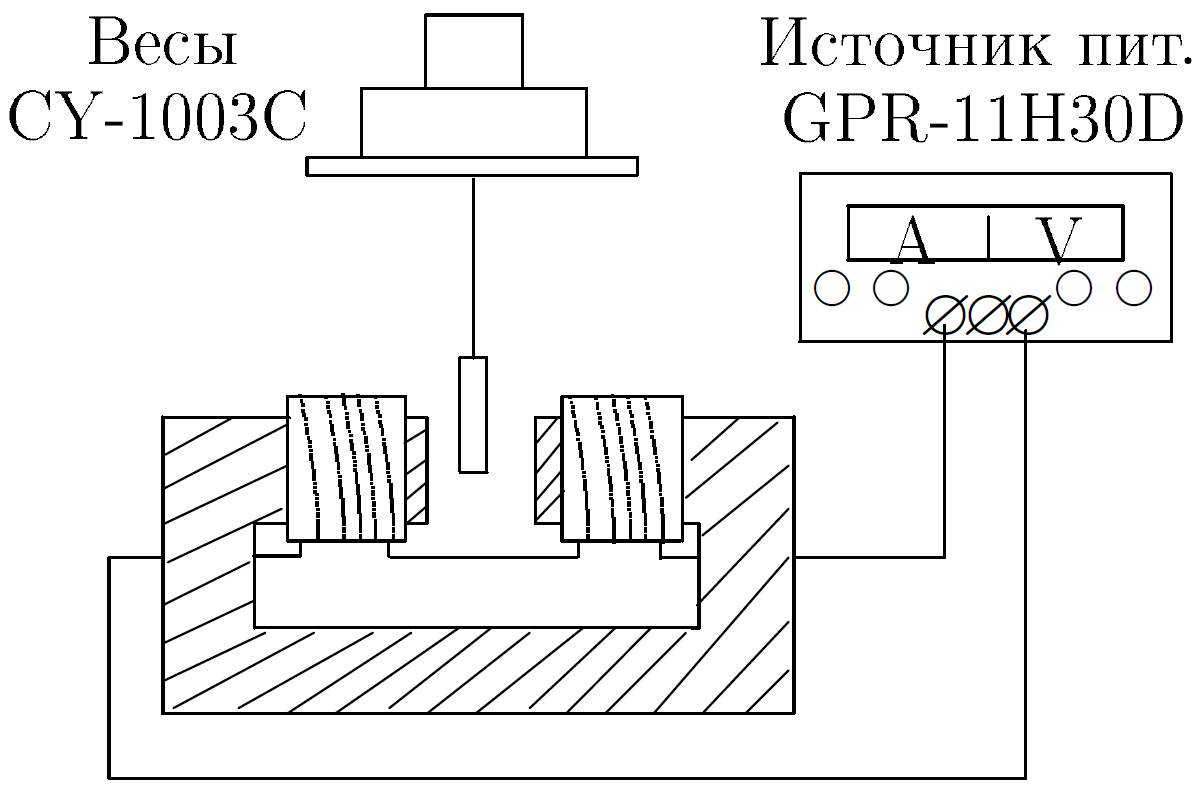
\includegraphics[width=6.5cm]{Screenshot_1.png}
	\caption{Схема экспериментальной установки.}
	\label{pic:1}
\end{wrapfigure}


Магнитное поле с максимальной индукцией $ \simeq 1 $ Т создаётся в зазоре электромагнита, питаемого постоянным током. Диаметр полюсов существенно превосходит ширину зазора, поэтому поле в средней части зазора достаточно однородно. Величина тока, проходящего через обмотки электромагнита, задаётся регулируемым источником питания GPR и измеряется амперметром $ А $, встроенным в источник питания. Градуировка электромагнита (связь между индукцией магнитного поля $ B $ в зазоре электромагнита и силой тока $ I $ в его обмотках) производится при помощи милливеберметра.


При измерениях образцы поочерёдно подвешиваются к весам так, что один конец образца оказывается в зазоре электромагнита, а другой -- вне зазора, где индукцией магнитного поля можно пренебречь. При помощи весов определяется перегрузка $ \Delta P = F $ -- сила, действующая на образец со стороны магнитного поля.


Силы, действующие на диа- и парамагнитные образцы, очень малы. Небольшие примеси ферромагнетиков (сотые доли процента железа или никеля) способны кардинально изменить результат опыта, поэтому образцы были специально отобраны.

\section{Ход работы}

\subsection{Градуировка электромагнита}

Сначала проведём градуировку магнита. Для этого используем тесламетр. С его помощью измерим значение магнитной индукции между полюсами электромагнита, изменяя ток от минимального до максимального значения с шагом в $ 0,1 $ А. Результаты измерений занесём в таблицу \ref{tab:my-table1}.

\begin{table}[H]
	\centering
	\begin{tabular}{|c|c|c|c|c|c|c|c|c|c|c|c|}
		\hline
		$ I $, А   & 0,1   & 0,2   & 0,3   & 0,4   & 0,5   & 0,6   & 0,7   & 0,8   & 0,9   & 1,0   & 1,1   \\ \hline
		$ B $, мТл & 103,5 & 200,8 & 300,5 & 403,8 & 496,1 & 605,9 & 680,9 & 758,8 & 830,9 & 890,1 & 951,6 \\ \hline
	\end{tabular}
	\caption{Результаты измерений}
	\label{tab:my-table1}
\end{table}

По полученным данным построим график зависимости $ B(I) $.

\begin{center}
	\begin{tikzpicture}
	\begin{axis}[
	title={График 1 \quad График зависимости $ B(I) $},
	xlabel={$ I $, А},
	ylabel={$B\cdot10^{-3}$, Тл},
	legend pos=north east,
	xmajorgrids=true,
	ymajorgrids=true,
	grid style=dashed,
	width = 520,
	height = 350,
	%xmin = 300,
	%xmax = 335,
	%ymin =40,
	%ymax =135,
	]
	\legend{ 
		,
		Аппроксимация зависимости,
	};
	\addplot+ [blue, only marks, mark size = 4pt,
	error bars/.cd,
	x dir=both, x explicit,
	y dir=both, y explicit, 
	] table [x = T, y = sigma] {
		T	sigma           
		0.1	103.5
		0.2	200.8
		0.3	300.5
		0.4	403.8
		0.5	496.1
		0.6	605.9
		0.7	680.9
		0.8	758.8
		0.9	830.9
		1.0	890.1
		1.1	951.6
	};
	\addplot [red, domain=0.08:1.1, line width =3.2pt] {48.42545+862.15455*x};
	\end{axis}
	\end{tikzpicture}
\end{center}

Аппроксимируем полученную зависимость уравнением вида $ y=kx+b $ при помощи программы OriginPro 2021. Результат аппроксимации также нанесём на график. В итоге получаем следующие результаты: 

\[ k = (862 \pm 27) \text{ } \frac{\text{мТл}}{\text{А}}, \]
\[ b = (48,4 \pm 18,2) \text{ мТл}. \]

\subsection{Измерение сил, действующих на образцы в магнитном поле}

При пулевом токе через электромагнит подвесим к весам один из образцов так, чтобы он не касался наконечников электромагнита. Обнулим показания весов, чтобы измерять непосредственно перегрузки $ \Delta P = F $ -- силы, действующей на образец при различных токах в обмотках электромагнита.


Установим минимальное из выбранных при калибровке магнита значение тока $ A_{min} $ и проведём измерение перегрузки. Повторим измерения $ \Delta P = f(I) $ для значений тока в диапазоне от $ A_{min} $ до $ A_{max} $. Также проведём серию измерений, уменьшая ток через магнит. Проведём такие измерения для различных образцов. Результаты измерений занесём в таблицу \ref{tab:my-table2}.

\begin{table}[H]
	\centering
	\resizebox{\textwidth}{!}{%
		\begin{tabular}{|cccc|cccc|cccc|}
			\hline
			\multicolumn{4}{|c|}{Al}                                                                  & \multicolumn{4}{c|}{Cu}                                                                    & \multicolumn{4}{c|}{графит}                                                                \\ \hline
			\multicolumn{2}{|c|}{$ \nearrow $}                        & \multicolumn{2}{c|}{$ \searrow $}   & \multicolumn{2}{c|}{$ \nearrow $}                         & \multicolumn{2}{c|}{$ \searrow $}    & \multicolumn{2}{c|}{$ \nearrow $}                         & \multicolumn{2}{c|}{$ \searrow $}    \\ \hline
			\multicolumn{1}{|c|}{$ I $, А}   & \multicolumn{1}{c|}{$ \Delta P $, $ \mu $Н}    & \multicolumn{1}{c|}{$ I $, А}   & $ \Delta P $, $ \mu $Н    & \multicolumn{1}{c|}{$ I $, А}   & \multicolumn{1}{c|}{$ \Delta P $, $ \mu $Н}     & \multicolumn{1}{c|}{$ I $, А}   & $ \Delta P $, $ \mu $Н     & \multicolumn{1}{c|}{$ I $, А}   & \multicolumn{1}{c|}{$ \Delta P $, $ \mu $Н}     & \multicolumn{1}{c|}{$ I $, А}   & $ \Delta P $, $ \mu $Н     \\ \hline
			\multicolumn{1}{|c|}{0,1} & \multicolumn{1}{c|}{9,8}   & \multicolumn{1}{c|}{0,1} & 9,8   & \multicolumn{1}{c|}{0,1} & \multicolumn{1}{c|}{-9,8}   & \multicolumn{1}{c|}{0,1} & -9,8   & \multicolumn{1}{c|}{0,1} & \multicolumn{1}{c|}{88,3}   & \multicolumn{1}{c|}{0,1} & 176,6  \\ \hline
			\multicolumn{1}{|c|}{0,2} & \multicolumn{1}{c|}{29,4}  & \multicolumn{1}{c|}{0,2} & 29,4  & \multicolumn{1}{c|}{0,2} & \multicolumn{1}{c|}{-19,6}  & \multicolumn{1}{c|}{0,2} & -29,4  & \multicolumn{1}{c|}{0,2} & \multicolumn{1}{c|}{343,4}  & \multicolumn{1}{c|}{0,2} & 470,9  \\ \hline
			\multicolumn{1}{|c|}{0,3} & \multicolumn{1}{c|}{58,9}  & \multicolumn{1}{c|}{0,3} & 68,7  & \multicolumn{1}{c|}{0,3} & \multicolumn{1}{c|}{-39,2}  & \multicolumn{1}{c|}{0,3} & -29,4  & \multicolumn{1}{c|}{0,3} & \multicolumn{1}{c|}{676,9}  & \multicolumn{1}{c|}{0,3} & 794,6  \\ \hline
			\multicolumn{1}{|c|}{0,4} & \multicolumn{1}{c|}{107,9} & \multicolumn{1}{c|}{0,4} & 117,7 & \multicolumn{1}{c|}{0,4} & \multicolumn{1}{c|}{-58,9}  & \multicolumn{1}{c|}{0,4} & -58,9  & \multicolumn{1}{c|}{0,4} & \multicolumn{1}{c|}{941,8}  & \multicolumn{1}{c|}{0,4} & 1020,2 \\ \hline
			\multicolumn{1}{|c|}{0,5} & \multicolumn{1}{c|}{166,8} & \multicolumn{1}{c|}{0,5} & 186,4 & \multicolumn{1}{c|}{0,5} & \multicolumn{1}{c|}{-88,3}  & \multicolumn{1}{c|}{0,5} & -88,3  & \multicolumn{1}{c|}{0,5} & \multicolumn{1}{c|}{1226,3} & \multicolumn{1}{c|}{0,5} & 1412,6 \\ \hline
			\multicolumn{1}{|c|}{0,6} & \multicolumn{1}{c|}{235,4} & \multicolumn{1}{c|}{0,6} & 235,4 & \multicolumn{1}{c|}{0,6} & \multicolumn{1}{c|}{-107,9} & \multicolumn{1}{c|}{0,6} & -107,9 & \multicolumn{1}{c|}{0,6} & \multicolumn{1}{c|}{1481,3} & \multicolumn{1}{c|}{0,6} & 1697,1 \\ \hline
			\multicolumn{1}{|c|}{0,7} & \multicolumn{1}{c|}{313,9} & \multicolumn{1}{c|}{0,7} & 284,5 & \multicolumn{1}{c|}{0,7} & \multicolumn{1}{c|}{-147,2} & \multicolumn{1}{c|}{0,7} & -147,2 & \multicolumn{1}{c|}{0,7} & \multicolumn{1}{c|}{1834,5} & \multicolumn{1}{c|}{0,7} & 1952,2 \\ \hline
			\multicolumn{1}{|c|}{0,8} & \multicolumn{1}{c|}{382,6} & \multicolumn{1}{c|}{0,8} & 412,0 & \multicolumn{1}{c|}{0,8} & \multicolumn{1}{c|}{-176,6} & \multicolumn{1}{c|}{0,8} & -186,4 & \multicolumn{1}{c|}{0,8} & \multicolumn{1}{c|}{2050,3} & \multicolumn{1}{c|}{0,8} & 2197,4 \\ \hline
			\multicolumn{1}{|c|}{0,9} & \multicolumn{1}{c|}{470,9} & \multicolumn{1}{c|}{0,9} & 510,1 & \multicolumn{1}{c|}{0,9} & \multicolumn{1}{c|}{-215,8} & \multicolumn{1}{c|}{0,9} & -235,4 & \multicolumn{1}{c|}{0,9} & \multicolumn{1}{c|}{2344,6} & \multicolumn{1}{c|}{0,9} & 2403,5 \\ \hline
			\multicolumn{1}{|c|}{1,0} & \multicolumn{1}{c|}{549,4} & \multicolumn{1}{c|}{1,0} & 569,0 & \multicolumn{1}{c|}{1,0} & \multicolumn{1}{c|}{-264,9} & \multicolumn{1}{c|}{1,0} & -274,7 & \multicolumn{1}{c|}{1,0} & \multicolumn{1}{c|}{2511,4} & \multicolumn{1}{c|}{1,0} & 2599,7 \\ \hline
			\multicolumn{1}{|c|}{1,1} & \multicolumn{1}{c|}{647,5} & \multicolumn{1}{c|}{1,1} & 647,5 & \multicolumn{1}{c|}{1,1} & \multicolumn{1}{c|}{-304,1} & \multicolumn{1}{c|}{1,1} & -304,1 & \multicolumn{1}{c|}{1,1} & \multicolumn{1}{c|}{2737,0} & \multicolumn{1}{c|}{1,1} & 2737,0 \\ \hline
		\end{tabular}%
	}
	\caption{Результаты измерений}
	\label{tab:my-table2}
\end{table}

Также построим графики зависимостей $ |\Delta P| = f(B^2) $. Для этого переведём $ I $ в $ B $ по градуировочным данным согласно таблице \ref{tab:my-table1}. Данные, полученные после обработки занесём в таблицу \ref{tab:my-table3}.

% Please add the following required packages to your document preamble:
% \usepackage{graphicx}
\begin{table}[H]
	\centering
	\resizebox{\textwidth}{!}{%
		\begin{tabular}{|cccc|cccc|cccc|}
			\hline
			\multicolumn{4}{|c|}{Al}                                                                                                                        & \multicolumn{4}{c|}{Cu}                                                                                                                        & \multicolumn{4}{c|}{графит}                                                                                                                    \\ \hline
			\multicolumn{2}{|c|}{$ \nearrow $}                                                & \multicolumn{2}{c|}{$ \searrow $}                           & \multicolumn{2}{c|}{$ \nearrow $}                                                & \multicolumn{2}{c|}{$ \searrow $}                           & \multicolumn{2}{c|}{$ \nearrow $}                                                & \multicolumn{2}{c|}{$ \searrow $}                           \\ \hline
			\multicolumn{1}{|c|}{$B^2$, Тл$^2$} & \multicolumn{1}{c|}{$ \Delta P $, $ \mu $Н} & \multicolumn{1}{c|}{$B^2$, Тл$^2$} & $ \Delta P $, $ \mu $Н & \multicolumn{1}{c|}{$B^2$, Тл$^2$} & \multicolumn{1}{c|}{$ \Delta P $, $ \mu $Н} & \multicolumn{1}{c|}{$B^2$, Тл$^2$} & $ \Delta P $, $ \mu $Н & \multicolumn{1}{c|}{$B^2$, Тл$^2$} & \multicolumn{1}{c|}{$ \Delta P $, $ \mu $Н} & \multicolumn{1}{c|}{$B^2$, Тл$^2$} & $ \Delta P $, $ \mu $Н \\ \hline
			\multicolumn{1}{|c|}{0,011}         & \multicolumn{1}{c|}{9,8}                    & \multicolumn{1}{c|}{0,011}         & 9,8                    & \multicolumn{1}{c|}{0,011}         & \multicolumn{1}{c|}{-9,8}                   & \multicolumn{1}{c|}{0,011}         & -9,8                   & \multicolumn{1}{c|}{0,011}         & \multicolumn{1}{c|}{88,3}                   & \multicolumn{1}{c|}{0,011}         & 176,6                  \\ \hline
			\multicolumn{1}{|c|}{0,040}         & \multicolumn{1}{c|}{29,4}                   & \multicolumn{1}{c|}{0,040}         & 29,4                   & \multicolumn{1}{c|}{0,040}         & \multicolumn{1}{c|}{-19,6}                  & \multicolumn{1}{c|}{0,040}         & -29,4                  & \multicolumn{1}{c|}{0,040}         & \multicolumn{1}{c|}{343,4}                  & \multicolumn{1}{c|}{0,040}         & 470,9                  \\ \hline
			\multicolumn{1}{|c|}{0,090}         & \multicolumn{1}{c|}{58,9}                   & \multicolumn{1}{c|}{0,090}         & 68,7                   & \multicolumn{1}{c|}{0,090}         & \multicolumn{1}{c|}{-39,2}                  & \multicolumn{1}{c|}{0,090}         & -29,4                  & \multicolumn{1}{c|}{0,090}         & \multicolumn{1}{c|}{676,9}                  & \multicolumn{1}{c|}{0,090}         & 794,6                  \\ \hline
			\multicolumn{1}{|c|}{0,163}         & \multicolumn{1}{c|}{107,9}                  & \multicolumn{1}{c|}{0,163}         & 117,7                  & \multicolumn{1}{c|}{0,163}         & \multicolumn{1}{c|}{-58,9}                  & \multicolumn{1}{c|}{0,163}         & -58,9                  & \multicolumn{1}{c|}{0,163}         & \multicolumn{1}{c|}{941,8}                  & \multicolumn{1}{c|}{0,163}         & 1020,2                 \\ \hline
			\multicolumn{1}{|c|}{0,246}         & \multicolumn{1}{c|}{166,8}                  & \multicolumn{1}{c|}{0,246}         & 186,4                  & \multicolumn{1}{c|}{0,246}         & \multicolumn{1}{c|}{-88,3}                  & \multicolumn{1}{c|}{0,246}         & -88,3                  & \multicolumn{1}{c|}{0,246}         & \multicolumn{1}{c|}{1226,3}                 & \multicolumn{1}{c|}{0,246}         & 1412,6                 \\ \hline
			\multicolumn{1}{|c|}{0,367}         & \multicolumn{1}{c|}{235,4}                  & \multicolumn{1}{c|}{0,367}         & 235,4                  & \multicolumn{1}{c|}{0,367}         & \multicolumn{1}{c|}{-107,9}                 & \multicolumn{1}{c|}{0,367}         & -107,9                 & \multicolumn{1}{c|}{0,367}         & \multicolumn{1}{c|}{1481,3}                 & \multicolumn{1}{c|}{0,367}         & 1697,1                 \\ \hline
			\multicolumn{1}{|c|}{0,464}         & \multicolumn{1}{c|}{313,9}                  & \multicolumn{1}{c|}{0,464}         & 284,5                  & \multicolumn{1}{c|}{0,464}         & \multicolumn{1}{c|}{-147,2}                 & \multicolumn{1}{c|}{0,464}         & -147,2                 & \multicolumn{1}{c|}{0,464}         & \multicolumn{1}{c|}{1834,5}                 & \multicolumn{1}{c|}{0,464}         & 1952,2                 \\ \hline
			\multicolumn{1}{|c|}{0,576}         & \multicolumn{1}{c|}{382,6}                  & \multicolumn{1}{c|}{0,576}         & 412,0                  & \multicolumn{1}{c|}{0,576}         & \multicolumn{1}{c|}{-176,6}                 & \multicolumn{1}{c|}{0,576}         & -186,4                 & \multicolumn{1}{c|}{0,576}         & \multicolumn{1}{c|}{2050,3}                 & \multicolumn{1}{c|}{0,576}         & 2197,4                 \\ \hline
			\multicolumn{1}{|c|}{0,690}         & \multicolumn{1}{c|}{470,9}                  & \multicolumn{1}{c|}{0,690}         & 510,1                  & \multicolumn{1}{c|}{0,690}         & \multicolumn{1}{c|}{-215,8}                 & \multicolumn{1}{c|}{0,690}         & -235,4                 & \multicolumn{1}{c|}{0,690}         & \multicolumn{1}{c|}{2344,6}                 & \multicolumn{1}{c|}{0,690}         & 2403,5                 \\ \hline
			\multicolumn{1}{|c|}{0,792}         & \multicolumn{1}{c|}{549,4}                  & \multicolumn{1}{c|}{0,792}         & 569,0                  & \multicolumn{1}{c|}{0,792}         & \multicolumn{1}{c|}{-264,9}                 & \multicolumn{1}{c|}{0,792}         & -274,7                 & \multicolumn{1}{c|}{0,792}         & \multicolumn{1}{c|}{2511,4}                 & \multicolumn{1}{c|}{0,792}         & 2599,7                 \\ \hline
			\multicolumn{1}{|c|}{0,906}         & \multicolumn{1}{c|}{647,5}                  & \multicolumn{1}{c|}{0,906}         & 647,5                  & \multicolumn{1}{c|}{0,906}         & \multicolumn{1}{c|}{-304,1}                 & \multicolumn{1}{c|}{0,906}         & -304,1                 & \multicolumn{1}{c|}{0,906}         & \multicolumn{1}{c|}{2737,0}                 & \multicolumn{1}{c|}{0,906}         & 2737,0                 \\ \hline
		\end{tabular}%
	}
	\caption{Данные для графиков}
	\label{tab:my-table3}
\end{table}

По этим данным построим графики зависимостей $ \Delta P(B^2) $ для различных исследуемых образцов.

\begin{center}
	\begin{tikzpicture}
	\begin{axis}[
	title={График 2.1 \quad График зависимости $ \Delta P(B^2) $ для алюминия},
	xlabel={$ B^2 $, Тл$ ^2 $},
	ylabel={$|\Delta P|$, $ \mu $Н},
	legend pos=north west,
	xmajorgrids=true,
	ymajorgrids=true,
	grid style=dashed,
	width = 520,
	height = 200,
	%xmin = 300,
	%xmax = 335,
	%ymin =40,
	%ymax =135,
	]
	\legend{ 
		$ \nearrow $,
		$ \searrow $,
		Аппроксимация зависимости,
	};
	\addplot+ [blue, only marks, mark size = 4pt,
	error bars/.cd,
	x dir=both, x explicit,
	y dir=both, y explicit, 
	] table [x = T, y = sigma] {
		T	sigma           
		0.011	9.8
		0.040	29.4
		0.090	58.9
		0.163	107.9
		0.246	166.8
		0.367	235.4
		0.464	313.9
		0.576	382.6
		0.690	470.9
		0.792	549.4
		0.906	647.5
	};
	\addplot+ [blue, only marks, mark size = 5pt, mark=triangle*,
	error bars/.cd,
	x dir=both, x explicit,
	y dir=both, y explicit, 
	] table [x = T, y = sigma] {
		T	sigma           
		0.011	9.8
		0.040	29.4
		0.090	68.7
		0.163	117.7
		0.246	186.4
		0.367	235.4
		0.464	284.5
		0.576	412.0
		0.690	510.1
		0.792	569.0
		0.906	647.5
	};
	\addplot [red, domain=0:0.95, line width =3.2pt] {699.59982*x};
	\end{axis}
	\end{tikzpicture}
\end{center}

\begin{center}
	\begin{tikzpicture}
	\begin{axis}[
	title={График 2.2 \quad График зависимости $ \Delta P(B^2) $ для меди},
	xlabel={$ B^2 $, Тл$ ^2 $},
	ylabel={$|\Delta P|$, $ \mu $Н},
	legend pos=north west,
	xmajorgrids=true,
	ymajorgrids=true,
	grid style=dashed,
	width = 520,
	height = 330,
	%xmin = 300,
	%xmax = 335,
	%ymin =40,
	%ymax =135,
	]
	\legend{ 
		$ \nearrow $,
		$ \searrow $,
		Аппроксимация зависимости,
	};
	\addplot+ [blue, only marks, mark size = 4pt,
	error bars/.cd,
	x dir=both, x explicit,
	y dir=both, y explicit, 
	] table [x = T, y = sigma] {
		T	sigma           
		0.011	9.81
		0.040	19.62
		0.090	39.24
		0.163	58.86
		0.246	88.29
		0.367	107.91
		0.464	147.15
		0.576	176.58
		0.690	215.82
		0.792	264.87
		0.906	304.11
	};
	\addplot+ [blue, only marks, mark size = 5pt, mark=triangle*,
	error bars/.cd,
	x dir=both, x explicit,
	y dir=both, y explicit, 
	] table [x = T, y = sigma] {
		T	sigma           
		0.011	9.81
		0.040	29.43
		0.090	29.43
		0.163	58.86
		0.246	88.29
		0.367	107.91
		0.464	147.15
		0.576	186.39
		0.690	235.44
		0.792	274.68
		0.906	304.11
	};
	\addplot [red, domain=0:0.95, line width =3.2pt] {330.32341*x};
	\end{axis}
	\end{tikzpicture}
\end{center}

\begin{center}
	\begin{tikzpicture}
	\begin{axis}[
	title={График 2.3 \quad График зависимости $ \Delta P(B^2) $ для графита},
	xlabel={$ B^2 $, Тл$ ^2 $},
	ylabel={$|\Delta P|$, $ \mu $Н},
	legend pos=north west,
	xmajorgrids=true,
	ymajorgrids=true,
	grid style=dashed,
	width = 520,
	height = 330,
	%xmin = 300,
	%xmax = 335,
	%ymin =40,
	%ymax =135,
	]
	\legend{ 
		$ \nearrow $,
		$ \searrow $,
		Аппроксимация зависимости,
	};
	\addplot+ [blue, only marks, mark size = 4pt,
	error bars/.cd,
	x dir=both, x explicit,
	y dir=both, y explicit, 
	] table [x = T, y = sigma] {
		T	sigma           
		0.011	88.3
		0.040	343.4
		0.090	676.9
		0.163	941.8
		0.246	1226.3
		0.367	1481.3
		0.464	1834.5
		0.576	2050.3
		0.690	2344.6
		0.792	2511.4
		0.906	2737.0
	};
	\addplot+ [blue, only marks, mark size = 5pt, mark=triangle*,
	error bars/.cd,
	x dir=both, x explicit,
	y dir=both, y explicit, 
	] table [x = T, y = sigma] {
		T	sigma           
		0.011	176.6
		0.040	470.9
		0.090	794.6
		0.163	1020.2
		0.246	1412.6
		0.367	1697.1
		0.464	1952.2
		0.576	2197.4
		0.690	2403.5
		0.792	2599.7
		0.906	2737.0
	};
	\addplot [red, domain=0:0.95, line width =3.2pt] {2777.9754*x + 434.33804};
	\end{axis}
	\end{tikzpicture}
\end{center}

Полученные графики аппроксимируем зависимости вида $ y = kx $ (для графита -- $ y = kx + b $) при помощи программы OriginLab 2021. Результаты аппроксимации занесём в таблицу \ref{tab:my-table4}.

% Please add the following required packages to your document preamble:
% \usepackage{graphicx}
\begin{table}[H]
	\centering	
	\begin{tabular}{|cc|cc|cc|}
		\hline
		\multicolumn{2}{|c|}{Al}                              & \multicolumn{2}{c|}{Cu}                               & \multicolumn{2}{c|}{графит}                           \\ \hline
		\multicolumn{1}{|c|}{$k$, $\mu$Н/Тл$^2$}        & 700 & \multicolumn{1}{c|}{$k$, $\mu$Н/Тл$^2$}        & -330 & \multicolumn{1}{c|}{$k$, $\mu$Н/Тл$^2$}        & 2778 \\ \hline
		\multicolumn{1}{|c|}{$\sigma_k$, $\mu$Н/Тл$^2$} & 23  & \multicolumn{1}{c|}{$\sigma_k$, $\mu$Н/Тл$^2$} & 19   & \multicolumn{1}{c|}{$\sigma_k$, $\mu$Н/Тл$^2$} & 385  \\ \hline
	\end{tabular}
	\caption{Результаты аппроксимации зависимостей}
	\label{tab:my-table4}
\end{table}

\subsection{Расчёт величины $ \chi $}

Согласно формуле \eqref{5}, вычислим коэффициент $ \chi $ для каждого образца. Из этой формулы следует, что

\begin{equation}\label{6}
k = \frac{\chi s}{2\mu_0}.
\end{equation}
Отсюда
\begin{equation}\label{7}
\boxed{\chi = \frac{2\mu_0 k}{s}}
\end{equation}
где $ s $ -- площадь поперечного сечения исследуемых образцов. В нашем случае $ s = (0,78 \pm 0,02) $ см$ ^2 $ для всех образцов.

Проводя вычисления, записываем итоговые результаты вычислений в таблицу \ref{tab:my-table5}.

\begin{table}[H]
	\centering
	\begin{tabular}{|c|c|c|c|}
		\hline
		образец  & Al   & Cu    & Графит \\ \hline
		$ \chi \cdot 10^{-5} $       & 2,24 & -1,06 & 8,89   \\ \hline
		$ \sigma_\chi \cdot 10^{-5} $ & 0,19 & 0,15  & 1,23   \\ \hline
	\end{tabular}
	\caption{Итоги}
	\label{tab:my-table5}
\end{table}

\section{Обсуждение результатов и выводы}

В ходе данной работы была измерена магнитная восприимчивость диа- и пара- магнетиков. Были исследованы образцы алюминия, меди и графита. Для алюминия и меди табличные значения магнитной восприимчивости равны \underline{$ \chi_{Al}^t = 2,3 \cdot 10^{-5} $} и \underline{$ \chi_{Cu}^t = -1,0 \cdot 10^{-5} $} соответственно. Полученные экспериментально данные совпадают с табличными в пределах погрешностей. Исходя из этого можно сказать, что алюминий является парамагнетиком $ (\chi > 0) $, а медь в свою очередь -- диамагнетиком $ (\chi < 0) $.


Результаты эксперимента для графика не столь однозначны. Несмотря на то, что графит должен демонстрировать диамагнетизм, в нашем опыте он обладает парамагнитными свойствами. Это могло произойти из-за того, что исследуемый образец имел недостаточную длину и не мог полностью оказаться между двух обкладок электромагнита. Вследствие этого могли возникнуть некоторые неточности в ходи измерения истинного поведения образца в магнитном поле. Кроме того, о неточности опытов также говорит нарушение линейности графика зависимости $ |\Delta P|(B^2) $. Поэтому полученные данные нельзя рассматривать как настоящие характеристика материала.


Таким образом, описанный выше метод измерения магнитной проницаемости материалов является рабочим и позволяет с хорошей точность определить эту величину для различных исследуемых образцов.

\end{document}